\textbf{📋 Apa yang akan dipelajari}

Pada bab ini kita akan mempelajari konsep Pemrograman Berorientasi Objek (OOP) dalam C++:

\begin{itemize}
\item Pengenalan OOP dan paradigma pemrograman
\item Konsep Class dan Object
\item Encapsulation dan data hiding
\item Method dan constructor
\end{itemize}

\minitoc

\section{🎯 Pemrograman Berorientasi Objek (OOP)}\label{pemrograman-berorientasi-obyek}

\subsection{Perbedaan C dan C++}

Bahasa C++ memiliki keunggulan dan perubahan yang besar dibandingkan dengan bahasa C. Salah satu perubahan mendasarnya adalah bahasa C++ dibuat untuk mendukung \textbf{pemrograman berorientasi objek}.

\subsection{Apa itu Paradigma Pemrograman?}

Paradigma pemrograman adalah cara pandang pemrogram terhadap eksekusi sebuah program:
\begin{itemize}
\item \textbf{OOP} - program adalah kumpulan objek yang saling berinteraksi
\item \textbf{Pemrograman terstruktur} - program adalah urutan instruksi yang dieksekusi berurutan
\end{itemize}

\subsection{Keunggulan OOP}

Pemrograman Berorientasi Objek adalah paradigma pemrograman yang sangat populer. Meskipun lebih baru dari pemrograman terstruktur, keduanya saling melengkapi.

\subsubsection{Kelebihan OOP}

\begin{itemize}
\item \textbf{Representasi dunia nyata} - membuat representasi teknis sedekat mungkin dengan pandangan konseptual dari dunia nyata
\item \textbf{Kerangka yang stabil} - membuat kerangka analisis dan spesifikasi yang stabil
\item \textbf{Mudah dikembangkan} - memudahkan pengembangan dan perubahan program
\end{itemize}

\subsection{Objek dalam Dunia Nyata}

Dunia ini penuh dengan objek. Contoh objek: sepeda, matahari, rumah, orang, anjing, topi, meja, dan masih banyak lagi.

\subsubsection{Karakteristik Objek}

\begin{itemize}
\item \textbf{Dapat dilihat} - objek memiliki bentuk fisik
\item \textbf{Dapat digunakan} - objek memiliki fungsi tertentu
\item \textbf{Memiliki ciri khas} - setiap objek memiliki karakteristik unik
\end{itemize}

\subsubsection{Contoh Objek Meja}

Objek meja tulis, meja makan, dan meja belajar memiliki ciri yang sama:
\begin{itemize}
\item Memiliki berat
\item Memiliki kaki meja
\item Memiliki warna meja
\end{itemize}

Objek meja juga dapat menerima operasi:
\begin{itemize}
\item Mengubah warna meja
\item Memotong atau menambah kaki meja
\end{itemize}

Jadi sebuah objek memiliki \textbf{sifat} yang melekat padanya dan \textbf{hal yang dapat dilakukan} terhadapnya.

\subsection{Konsep OOP dalam Pemrograman}

Pemrograman berorientasi objek adalah cara untuk mengorganisasikan program ke dalam komponen logis (kelas), yang saat digunakan harus diinstansiasi menjadi objek.

\subsubsection{Komponen OOP}

\begin{itemize}
\item \textbf{Kelas} - blueprint/template untuk membuat objek
\item \textbf{Objek} - instance/realisasi dari kelas
\item \textbf{Data member} - variabel yang menyimpan data
\item \textbf{Method} - fungsi yang bekerja dengan data tersebut
\end{itemize}

\subsubsection{Keunggulan OOP}

\begin{itemize}
\item \textbf{Fleksibel} - kode program lebih fleksibel
\item \textbf{Mudah dipelihara} - program lebih mudah dipelihara
\item \textbf{Encapsulation} - data dan prosedur dikemas dalam objek
\item \textbf{Abstraction} - pengguna tidak melihat proses internal objek
\end{itemize}

\section{🏗️ Kelas (Class)}\label{kelas}

\subsection{Apa itu Kelas?}

Kelas adalah \textbf{blueprint} dari objek, yaitu prototype yang mendefinisikan variabel-variabel dan method-method secara umum.

\subsection{Karakteristik Kelas}

\begin{itemize}
\item \textbf{Template} - kelas adalah template untuk membuat objek
\item \textbf{Instansiasi} - kelas harus diinstansiasi menjadi objek untuk digunakan
\item \textbf{Konsistensi} - setiap objek dari kelas yang sama memiliki sifat dan tingkah laku yang sama
\end{itemize}

\subsection{Struktur Kelas C++}

Secara umum, ada dua bagian utama pada sebuah class C++:
\begin{itemize}
\item \textbf{Class declaration} - mendefinisikan nama class dan atributnya
\item \textbf{Class body} - mendeklarasikan variabel dan method
\end{itemize}

\section{🎯 Objek (Object)}\label{object}

\subsection{Apa itu Objek?}

Objek adalah pengenal (identifier) yang menyatukan atribut (property/state) dengan tingkah laku (behaviour/method).

\subsection{Encapsulation}

Penyatuan State dan Behaviour ini pada konsep OOP disebut dengan istilah \textbf{encapsulation} (enkapsulasi).

\subsection{Karakteristik Objek}

Objek mempunyai dua karakteristik utama:
\begin{itemize}
\item \textbf{Atribut (State)} - status/keadaan objek
\item \textbf{Tingkah laku (Behaviour)} - method/fungsi yang dapat dilakukan objek
\end{itemize}

\textbf{Contoh:}

Object Sepeda

\begin{itemize}

\item
  Object Sepeda memiliki attribut (state) : pedal, roda, jeruji, warna,
  stang, jumlah roda.
\item
  Object Sepeda memiliki tingkah laku (behaviour): kecepatan menaik,
  kecepatan menurun, memberhentikan, menjalankan, mengganti gigi.
\end{itemize}

\section{Class dan Object}\label{class-dan-object-1}

Sering ada pertanyaan, class dan obyek duluan yang mana? Padahal
kenyataannya: class adalah blueprint/prototype saja. Class merupakan
definisi tentang state dan behaviour suatu objek. Bisa juga disebut
class adalah kumpulan object yang memiliki atribut dan service yang
sama. Sedangkan object adalah ``barang nyata'' dari sebuah class.

\textbf{Contoh class:} manusia sedangkan object-nya adalah kita, misalnya: Anton,
Rudi, dan Amir.

Class memiliki sifat pewarisan, yang berarti sifat dari satu class dapat
diturunkan ke class lain. Contoh pewarisan adalah class dosen memiliki
semua atribut/state dan services dari class manusia. Dari contoh di
atas, dapat dikatakan bahwa class dosen mewarisi semua atribut dan
service dari class manusia. Class manusia adalah class induk, class
dosen adalah class anak.

\section{Pembuatan Class pada C++}\label{pembuatan-class-pada-c}

Class pada C++ bisa dianggap sebagai tipe data baru. Selain tipe data
yang sudah dibawakan oleh C++, kita juga dapat membuat tipe data baru.
Jika pada bahasa C/C++ tipe data baru dibuat menggunakan struct, pada
C++ tipe data baru bisa dibuat dengan menggunakan class. Konsep ini
merupakan konsep berorientasi obyek.

Struktur sederhana sebuah class pada C++:

\lstinputlisting[language=c++]{../code/06-class-object-code-1.c++}

Contoh class:

\lstinputlisting[language=c++]{../code/06-class-object-code-2.c++}

\begin{quotation}
{\LARGE \ding{46}} 		\textbf{TIPS}

\begin{itemize}
\item Untuk membuat
nama class, biasakanlah menggunakan huruf besar.
				
\textbf{ Contohnya:}
				
 Kucing,Rumah, Handphone, dan lain-lain.
				
\item Untuk membuat nama
variabel biasakanlah menggunakan nama yang mewakili property yang
dimiliki dan melekat pada nama kelasnya. Pada contoh diatas, class
Kucing memiliki berat, umur, dan nama yang melekat erat padanya. Setiap
kucing yang ada didunia ini pada umumnya memiliki berat, umur, dan nama
yang berbeda-beda satu sama lain. Untuk menamai member variabel, jika
nama variabel hanya terdiri dari satu kata gunakanlah huruf kecil,
sedangkan jika terdiri dari lebih dari satu kata, gunakan huruf kecil
pada huruf kata pertama, sedangkan untuk kata selanjutnya gunakan huruf
besar pada huruf-huruf pertamanya.
				
 \textbf{Contoh: }string namaKucing, float
ipkMahasiswa, int berat, dan lain-lain.
				
\item Untuk membuat
nama member function, gunakanlah cara penulisan yang tepat untuk
menggambarkan secara benar setiap nama function yang ada. Biasakanlah
memberi nama function sesuai dengan behaviour yang memang dikerjakannya.
Contohnya: \texttt{void\ cariData(string\ judul)}, atau
				\texttt{int\ ambilNilai()} dan lain-lain.
			\end{itemize}
			
	\end{quotation}


\section{Mendefinisikan Obyek}\label{mendefinisikan-obyek}

Setelah kita selesai membuat class baru, maka kita bisa menggunakan
class tersebut adalah dengan menginisialisasinya (dengan membuat sebuah
atau beberapa obyek) dari class tersebut. Membuat obyek bisa dianggap
seperti membuat variabel yang bertipe class yang kita buat. Contoh:

\lstinputlisting[language=c++]{../code/06-class-object-code-3.c++}

Class dan obyek adalah berbeda. Class merupakan template dari member
variabel dan member function yang dapat dibuat wujud nyatanya dalam
sebuah obyek. Pada contoh diatas, Kucing adalah class. Kucing tidak bisa
langsung digunakan dalam program. Untuk bisa menggunakan Kucing, yang
harus dilakukan adalah membuat obyeknya, yaitu kucingku. Pada dunia
nyata kucingku bisa disebut sesuai dengan nama kucing yang kia pelihara.
Jadi contoh diatas mungkin bisa diubah menjadi Kucing katty. Dimana
katty adalah obyek dari class Kucing yang dapat digunakan dalam program.

\section{Mengakses Member Variabel}\label{mengakses-member-variabel}

Setelah kita membuat obyek seperti:

\lstinputlisting[language=c++]{../code/06-class-object-code-4.c++}

Cara mengakses member variabel adalah dengan menggunakan tanda titik
(.). Contoh jika kita hendak mengisi data berat badan katty dengan nilai
8 kg, maka yang harus dilakukan adalah:

\lstinputlisting[language=c++]{../code/06-class-object-code-5.c++}

Demikian juga dengan nama, umur, dan jenis kelamin.

\lstinputlisting[language=c++]{../code/06-class-object-code-6.c++}

\section{Mengakses Member
Function/Method}\label{mengakses-member-functionmethod}

Sedangkan cara untuk mengakses member function dari suatu class adalah
dengan juga menggunakan tanda titik pada obyeknya. Contoh:

\lstinputlisting[language=c++]{../code/06-class-object-code-7.c++}

\subsubsection*{Contoh  Pembuatan class Sepeda}

Buatlah project baru dan tulis kode berikut:

\lstinputlisting[language=c++, caption=Pembuatan class Sepeda, label=contoh6-1]{../code/06-class-object-contoh6-1.c++}

\textbf{Hasil:}

\begin{lcverbatim}
Kecepatan: 30 Merk: Federal
\end{lcverbatim}

\textbf{Keterangan:}

\begin{itemize}

\item
  Program diatas membuat sebuah class bernama Sepeda. Di dalam class
  Sepeda, terdapat dua bagian, bagian pertama berisi semua member
  variabel yang bersifat private, yaitu kecepatan, gigi, dan merk. Pada
  bagian kedua terdapat member function yang hanya beisi judul method
  saja sedangkan implementasinya diletakkan diluar class Sepeda.
\item
  Diluar kelas Sepeda, kita mendefinisikan semua implementasi method
  dari semua member function yang sudah kita definisikan diatas. Untuk
  mengakses member function dari luar kelasnya, digunakan tanda
  \texttt{::} setelah nama class. Implementasi method bisa menggunakan
  cara lain yang akan dijelaskan dibagian-bagian berikutnya.
\item
  Pada function main, kita membuat obyek dari class Sepeda yang bernama
  objSpd dan kemudian kita akses semua member functionnya.
\item
  Sebelum menampilkan hasil kita isi terlebih dahulu kecepatan, gigi,
  dan merk dari Sepeda yang kita buat.
\item
  Keyword this mengacu pada class itu sendiri (class Sepeda) dan
  merupakan variabel pointer. Keyword tersebut digunakan untuk mengakses
  semua member variabel dan member method class Sepeda.
\end{itemize}
\begin{quotation}
{\LARGE \ding{46}} 	\textbf{TIPS} 
	
	Keyword
	\texttt{this} pada class Sepeda merupakan kata kunci untuk mengakses
	class yang didefinisikan (kelas dirinya sendiri). Tanda
	\texttt{-\textgreater{}} merupakan tanda bahwa \texttt{this} merupakan
	obyek pointer. Cara lain untuk mengakses kelas itu sendiri adalah dengan
	menggunakan \texttt{\textless{}namakelas\textgreater{}::} diikuti nama
	method / variabel member .
\end{quotation}
 
 
  

Contoh :

\lstinputlisting[language=c++]{../code/06-class-object-code-9.c++}

\subsubsection*{Contoh  Pembuatan obyek Sepeda.}

Buatlah project baru dan tulis kode berikut:

\lstinputlisting[language=c++, caption=Pembuatan obyek Sepeda, label=contoh6-2]{../code/06-class-object-contoh6-2.c++}

\textbf{Hasil:}

\begin{lcverbatim}
Sepeda pertama:
Kecepatan: 30
Merk: Federal
Gigi: 2
Sepeda kedua:
Kecepatan: 45
Merk: Polygon
\end{lcverbatim}

\textbf{Keterangan:}

\begin{itemize}

\item
  Program diatas merupakan pengembangan dari program sebelumnya dimana
  kita membuat satu lagi variabel \texttt{objSpd2}.
\item
  Terlihat bahwa masing-masing obyek sepeda yang terbuat memiliki data
  yang berbeda-beda satu sama lain.
\item
  Artinya class hanyalah merupakan template / blueprint saja, dimana
  data-data dan tingkah laku dari kelas haruslah dilakukan oleh
  obyeknya. Jadi obyek adalah bentuk nyata dari sebuah kelas yang
  memiliki data dan method yang berbeda-beda satu sama lain.
\end{itemize}

\subsubsection*{Contoh  Pembuatan Obyek Array Sepeda}

Buatlah program beikut ini:

\lstinputlisting[language=c++, caption=Pembuatan Obyek Array Sepeda, label=contoh6-3]{../code/06-class-object-contoh6-3.c++}

\textbf{Hasil:}
\begin{lcverbatim}
Sepeda pertama:
Tampilan Sepeda ke-1
Kecepatan: 30
Merk: Merk-
Gigi: 10
Tampilan Sepeda ke-2
Kecepatan: 31
Merk: erk-
Gigi: 11
Tampilan Sepeda ke-3
Kecepatan: 32
Merk: rk-
Gigi: 12
Tampilan Sepeda ke-4
Kecepatan: 33
Merk: k-
Gigi: 13
Tampilan Sepeda ke-5
Kecepatan: 34
Merk: -
Gigi: 14
\end{lcverbatim}

\textbf{Keterangan:}

\begin{itemize}

\item
  Program diatas merupakan pengembangan lagi dari Contoh \ref{contoh6-3}.
\item
  Program diatas membuat obyek dari class Sepeda dalam bentuk Array 1
  dimensi yang bertipe Sepeda.
\item
  Array yang bertipe class Sepeda tersebut tetap memiliki indeks dari 0
  sampai dengan n-1
\item
  Masing-masing obyek elemen array \texttt{objSpdArray} berisi data-data
  yang berbeda-beda satu sama lainnya.
\end{itemize}

\begin{quotation}
{\LARGE \ding{46}} 	\textbf{TIPS}
	
	Kita juga
	dapat melakukan assigment / penugasan terhadap obyek ke obyek lain.
	Contoh kita memiliki class Sepeda dan kita membuat obyek spd1 dan spd2.
	
	\begin{lstlisting}[language=c++, numbers=none]
	Sepeda spd1,spd2;
	spd1.setMerk("X");
	spd1.ubahKecepatan(50);
	spd1.ubahGigi(4);
	\end{lstlisting}
	
	maka bisa dilakukan:
	
	\begin{lstlisting}[language=c++, numbers=none]
	spd2 = spd1;
	\end{lstlisting}
	
	Jika \texttt{spd2} ditampilkan, dengan \texttt{sp2.tampilSepeda()}, maka
	nilai yang ditampilkan akan sama persis dengan nilai \texttt{spd1}.
\end{quotation}


Class yang kita definisikan memiliki member method. Semua member method
tersebut dapat kita gunakan. Apa yang kita buat dalam member method akan
membuat kompiler mendaftarkan semua method yang kita buat kedalam memory
sehingga hanya method yang kita daftarkan saja yang bisa kita akses dari
class kita.

\section{Hak Akses Member Variabel dan Method
Variabel}\label{hak-akses-member-variabel-dan-method-variabel}

Pada pemrograman berorientasi obyek, terdapat konsep penting yang
bernama \emph{enkapsulasi}. Konsep tersebut berarti kita ``membungkus''
semua member variabel dan member method kedalam suatu class termasuk hak
akses terhadap mereka. Apa arti hak akses? Hak akses adalah bagaimana
class yang terenkapsulasi tersebut ``menyembunyikan'' hal-hal yang tidak
perlu / tidak boleh dilihat dari luar class. Dengan adanya hak akses
tersebut semua data dan method akan terlindungi dan tidak termodifikasi.
Kita dapat analogikan dengan kasus nyata sebuah benda, misalnya AC. AC
merupakan alat elektronik yang rumit dan mampu mendinginkan ruangan.
Jika seseorang memasang AC maka AC akan melindungi dirinya dengan hak
akses. Kita sebagai orang awam tentang AC hanya diperbolehkan mengakses
yang diperbolehkan saja untuk mengantisipasi hal-hal yang tidak
diinginkan seperti misalnya AC akan rusak. Kita hanya diberikan
tombol-tombol sederhana dan mungkin remote untuk mengatur semua tentang
AC, kita tidak bisa mengakses hardwarenya, kabel didalamnya, PCB nya,
kondensatornya dan lain-lain. Yang bisa melakukan itu adalah para ahli
AC. Dengan demikian AC sudah berusaha melindungi dirinya dari
tangan-tangan orang awam yang memang tidak berhak.

Demikian pula pada class, class juga memiliki dua bagian: member
variabel dan member method. Kedua bagian ini berbeda fungsinya. Member
variabel digunakan untuk menyimpan sifat-sifat yang dimiliki dan melekat
pada class sedangkan method digunakan untuk melakukan operasi/kegiatan
terhadap class tersebut. Jika kita bandingan dengan AC, maka method bisa
dibilang sebagai remote/tombol. Sehingga untuk mengakses data-data yang
ada pada class kita sangat direkomendasikan untuk menggunakan method
bukan mengaksesnya secara langsung.

Class pada C++ memiliki cara melindungi dirinya yaitu dengan menggunakan
keyword private, protected dan public. Keyword private atau protected
biasanya digunakan pada semua variabel member sedangkan keyword
protected atau public digunakan pada semua variabel method. Dengan
menggunakan keyword private, maka bagian private tersebut tidak akan
bisa diakses dari luar class, harus dari dalam class tersebut atau
berada dalam method class tersebut, sedangkan jika public maka bisa
akses dari luar class.

\subsubsection*{Contoh  Perbedaan private dan public pada member variabel}
\begin{enumerate}
	

	\item Buatlah program berikut:
	
\lstinputlisting[language=c++, caption=Public pada member variabel, label=contoh6-4]{../code/06-class-object-contoh6-4.c++}
	
\item 	\textbf{Hasil:}
	
	\begin{lcverbatim}
Pengaksesan public:
Gigi: 3
Kecepatan: 30
Merk: Polygon
	\end{lcverbatim}
	
\item 	\textbf{Keterangan:}
	
	Semua variabel member yang bersifat public dapat diakses dan diisi
	dengan baik dari luar class, dalam hal ini adalah function
	\texttt{int\ main()}. Function \texttt{int\ main()} berada diluar class
	Sepeda Akan terjadi hal yang berbeda jika kita mengakses semua variabel
	member yang bersifat private.
	
\item 	Ubahlah program pada Contoh \ref{contoh6-4} diatas menjadi seperti berikut ini:
	
\lstinputlisting[language=c++, caption=Privat pada member variabel, label=contoh6-5]{../code/06-class-object-contoh6-5.c++}
	
\item 	\textbf{Hasil:}
	
	\begin{figure}[htbp]
		\centering
\shadowimage[width=8cm]{Capture6-1}

	\end{figure}
	
\item 	\textbf{Keterangan:}
	
	Akan terjadi compile time error, karena kita mengakses variabel member
	yang bersifat \emph{private}. Berarti class Sepeda sudah bisa menerapkan
	fungsi enkapsulasi dan melindungi data-datanya dari pengaksesan
	langsung.
\end{enumerate}




\section{Member Function / Member
Method}\label{member-function-member-method}

Seperti yang sudah dijelaskan, member method merupakan bagian yang harus
dideklarasikan sebagai bagian public. Salah satu kegunaan member
function adalah mengakses semua member variabel dan tetap mendukung
enkapsulasi. Cara untuk membuat member method adalah dengan
mendeklarasikannya pada bagian public, sedangkan implementasi kodingnya
berada diluar kelas. Berikut adalah contohya.

\lstinputlisting[language=c++]{../code/06-class-object-code-16.c++}

Di dalam pemrograman beriorientasi obyek pada umumnya member function
minimal selalu mewakili semua member variabelnya. Misal kita memiliki 1
buah member variabel bernama umur, maka minimal kita akan memiliki satu
buah member function, misalnya bernama ubahUmur(int u).

\subsubsection*{Contoh  Member function dan implementasinya.}

Buatlah program berikut ini:

\lstinputlisting[language=c++, caption=Member function dan implementasinya, label=contoh6-6]{../code/06-class-object-contoh6-6.c++}

\textbf{Hasil:}
\begin{lcverbatim}
Kecepatan: 30
Merk: Federal
\end{lcverbatim}


\textbf{Keterangan:}

\begin{itemize}

\item
  Semua member variabel yang dimiliki tidak diakses secara langsung dari
  function main, tapi melalui method-methodnya.
\item
  Pada program diatas setiap member variabel memiliki minimal satu buah
  method member
\item
  Terdapat satu buah method tambahan yang berfungsi untuk menampilkan
  semua informasi mengenai sepeda
\item
  Setiap method member dapat menerima input dan mengeluarkan output.
\item
  Kata kunci \texttt{this-\textgreater{}} pada method member berfungsi
  untuk mengakses semua member variabel yang terdapat pada class Sepeda
  yang biasanya bersifat private.
\item
  Implementasi method member berada diluar class Sepeda dan dimulai
  dengan nama classnya kemudian diikuti tanda :: yang artinya mengakses
  member method.
\end{itemize}

\section{Accessor dan Mutator
Method}\label{accessor-dan-mutator-method}

Pada pemrograman berorientasi obyek dengan C++, kita memiliki method
member. Tujuan dari method member selain memberi tingkah laku dari class
tersebut adalah melakukan akses terhadap semua member variabel yang
bersifat private agar tetap bisa diakses dari luar class.

Member method yang berkaitan dengan member variabel ada 2 jenis, yaitu
member method yang berfungsi untuk mengeset / mengisi nilai member
variabel dan member method yang berfungsi untuk mengambil nilai member
variabel.

\subsection{Accessor method}\label{accessor-method}

method ini berfungsi untuk mengambil nilai dari sebuah member variabel.
Asesor method biasanya dinamai :

\lstinputlisting[language=c++]{../code/06-class-object-code-18.c++}

\textbf{Contoh:}

\lstinputlisting[language=c++]{../code/06-class-object-code-19.c++}

\subsection{Mutator method}\label{mutator-method}

method ini berfungsi untuk mengisi / mengeset nilai kepada sebuah member
variabel

Mutator method biasanya dinamai :

\lstinputlisting[language=c++]{../code/06-class-object-code-20.c++}

\textbf{Contoh:}

\lstinputlisting[language=c++]{../code/06-class-object-code-21.c++}

\subsubsection*{Contoh  Penggunaan accessor dan mutator method}

Tulislah program berikut ini:

\lstinputlisting[language=c++, caption=Penggunaan accessor dan mutator method, label=contoh6-7]{../code/06-class-object-contoh6-7.c++}

\textbf{Hasil:}
\begin{lstlisting}
	Kucingku bernama Katty,
	dia berbobot 4 kg dan sudah berumur 2 tahun sekarang.
\end{lstlisting}
 

\textbf{Keterangan:}

\begin{itemize}

\item
  Program diatas memperlihatkan bagaimana setiap member variabel
  memiliki tepat dua buah method member, dimana setiap method member
  yang satu berfungsi sebagai asesor method dan yang lain berfungsi
  sebagai mutator method.
\item
  Terdapat sebuah method tambahan yaitu berlari yang hendak
  menggambarkan bahwa selain asesor dan mutator kita masih diperbolehkan
  membuat method lainnya.
\item
  Asesor method mengambil data member variabel sehingga dibuat fungsi
  berupa function non void, sedangkan mutator method mengeset data
  member variabel sehingga dibuat fungsi berupa function void yang
  menerima parameter yang sesuai dengan tipe data member variabelnya.
\end{itemize}

\section{Constructor dan
Destructor}\label{constructor-dan-destructor}

Kita dapat mendeklarasikan variabel biasa dan kemudian melakukan
inisialisasi terhadap variabel tersebut dengan mudah. Contoh:

\lstinputlisting[language=c++]{../code/06-class-object-code-24.c++}

Inisialisasi variabel berfungsi untuk mengisi suatu nilai awal terhadap
suatu variabel yang kita deklarasikan. Variabel tersebut masih bisa kita
ubah-ubah lagi nilainya dikemudian waktu. Nah bagaimana untuk
menginisialisasi variabel member pada suatu class? Caranya dengan
membuat method yang berjenis constructor method. Sedangkan untuk
mendealokasi dan melakukan finalisasi sebuah class kita gunakan
destructor method. Constructor berfungsi untuk menginisialisasi obyek
dari class dan mempersiapkan ruang memory, sedangkan destructor
menghapus dan membersihkan obyek ketika sudah tidak terpakai dan
membebaskan memory yang tadinya terpakai.

Constructor method merupakan method yang namanya sama dengan nama
classnya dan bersifat public tapi tidak berjenis void ataupun non void.
Constructor dapat menerima parameter namun tidak bisa mengembalikan
nilai apapun.

Desktruktor method merupakan method kebalikan dari constructor yang juga
bernama sama dengan nama classnya namun diawali dengan tanda
\textasciitilde{}. Destructor tidak boleh memiliki parameter apapun.

Contoh jika kita memiliki class bernama Sepeda, maka kita dapat membuat
constructor dengan nama Sepeda() juga. Sedangkan destructor method sama
dengan constructor namun diawali dengan tanda \texttt{\textasciitilde{}}
didepannya. Contoh:

\lstinputlisting[language=c++]{../code/06-class-object-code-25.c++}

\subsection{Default Constructor}\label{default-constructor}

Pada bahasa C++ semua class yang telah dibuat PASTI memiliki constructor
walaupun tidak kita buat. Compiler bahasa C++ pasti membuatnya walau
secara implisit. Constructor yang bernama sama dengan nama classnya dan
tidak berparameter disebut default constructor. Secara default pasti
semua class ada default constructornya. Kapan kita menggunakan
constructor? Setiap kali kita membuat obyek baru (melakukan instansiasi
obyek), maka kita memanggil constructor default.

\textbf{Contoh:}

\lstinputlisting[language=c++]{../code/06-class-object-code-26.c++}

Berarti kita memanggil default konstruktor bernama Sepeda() tanpa
parameter apapun. Jika kita membuat konsruktor dengan menggunakan
parameter seperti misalnya:

\lstinputlisting[language=c++]{../code/06-class-object-code-27.c++}

Maka pada saat instansiasi kita menggunakan cara sebagai berikut:

\lstinputlisting[language=c++]{../code/06-class-object-code-28.c++}

Arti instasiasi diatas adalah kita memanggil konstruktor yang
berparameter dua buah, string dan integer.

\subsubsection*{Contoh  Menggunakan Constructor dan Destructor.}

Buatlah program berikut:

\lstinputlisting[language=c++, caption=Menggunakan Constructor dan Destructor, label=contoh6-8]{../code/06-class-object-contoh6-8.c++}

\textbf{Hasil:}
\begin{lstlisting}
	Kucingku bernama Katty, dia berbobot 4 kg dan sudah
	berumur 2 tahun sekarang.
\end{lstlisting}
 

\textbf{Keterangan:}

\begin{itemize}

\item
  Program diatas menunjukkan pemakaian konstruktor dan desktruktor.
  Constructor digunakan untuk menginisialisasi umur kucing pada saat
  awal pertama obyek dibuat, kemudian pada akhirnya kita juga tetap
  dapat mengubah umur kucing dibagian akhir program.
\item
  Destruktor yang kita buat merupakan default desktruktor dimana
  desktruktor tidak boleh memiliki parameter apapun.
\end{itemize}

\begin{quotation}
{\LARGE \ding{46}} 	\textbf{TIPS} 
	
	Jika kita
	sudah membuat konstruktor yang memiliki parameter pada class kita, maka
	secara otomatis default constructor yang dibuat oleh compiler tidak ada
	lagi, sehingga ketika kita melakukan instansiasi pada class Kucing
	diatas tanpa parameter pasti akan error.
\end{quotation}


Contoh, tambahkan satu baris berikut ini pada bagian akhir kode pada
Contoh \ref{contoh6-1} sebelum \texttt{return\ a.exec()}.

\lstinputlisting[language=c++]{../code/06-class-object-code-31.c++}

Ketika dilakukan kompilasi akan menghasilkan error sebagai berikut:

\begin{figure}[htbp]
\centering
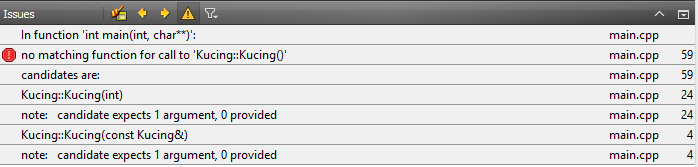
\includegraphics[width=0.8\textwidth]{Capture6-2}

\end{figure}

Error diatas mengatakan bahwa class Kucing tidak memiliki function yang
bernama \texttt{Kucing::Kucing()}, yang artinya method constructor
defaultnya sudah hilang. Agar kita dapat menggunakan baris
\texttt{Kucing\ kucingku2;} maka kita harus menambah method constructor
lagi yang tidak berparameter.

\subsubsection*{Contoh  Percobaan Menambah Constructor Method.}

Buatlah program berikut:

\lstinputlisting[language=c++, caption=Percobaan Menambah Constructor Method, label=contoh6-9]{../code/06-class-object-contoh6-9.c++}

\textbf{Hasil:}

\begin{lcverbatim}
Kucingku bernama Katty, dia berbobot 4 kg dan 
sudah berumur 2 tahun sekarang.
Lima tahun telah berlalu, sekarang kucingku 
sudah berumur:7 tahun
\end{lcverbatim}

\textbf{Keterangan:}

\begin{itemize}

\item
  Pada program C++, kita dapat membuat konstruktor method lebih dari
  satu, asal tidak sama. Konsep diatas dinamakan dengan polymorfisme
  (OVERLOADING) yang akan dibahas lebih lanjut dibab-bab berikutnya.
\item
  Dengan mendefinisikan konstruktor tanpa parameter maka kita dapat
  menginstansiasi obyek dengan cara biasa, seperti pada contoh Kucing
  kucingku2;
\end{itemize}

\subsection{Constructor Dengan nilai
Default}\label{constructor-dengan-nilai-default}

Constructor dapat memiliki nilai default sehingga jika konstruktor yang
dipanggil tidak diisi nilai, maka nilai-nilai lainnya akan tetap
diinisialisasi dengan nilai defaultnya. Hal ini diperlukan untuk
mempermudah menginisialisasi data variabel member. Penggunaan nilai
default ini juga memungkinkan kita untuk tidak memasukkan semua
parameter pada pemanggilan konstruktor.

\subsubsection*{Contoh  Penggunaan Constructor dengan Nilai Default}

Buatlah program berikut:

\lstinputlisting[language=c++, caption=Penggunaan Constructor dengan Nilai Default, label=contoh6-10]{../code/06-class-object-contoh6-10.c++}

\textbf{Hasil:}

\begin{lcverbatim}
Judul: unknown
Pengarang: unknown
Jumlah halaman: 1
Judul: unknown
Pengarang: Antonius
Jumlah halaman: 1
Judul: Membuat aplikasi C++
Pengarang: Robert
Jumlah halaman: 1
Judul: Pemrograman C
Pengarang: Walter
Jumlah halaman: 100
\end{lcverbatim}
\textbf{Keterangan:}

\begin{itemize}

\item
  Program diatas menunukkan bahwa kita dapat membuat konstruktor dengan
  nilai default, yaitu dengan menggunakan parameter dan langsung
  diinisialisasi dengan menggunakan tanda sama dengan (=).
\item
  Pada pemanggilan konstruktor, terlihat bahwa jika konstruktor tidak
  diisi parameter apapun maka ketika data ditampilkan semua isi member
  variabel sesuai dengan nilai defaultnya.
\item
  Pada pemanggilan konstruktor kedua, yaitu dengan satu parameter
  string, maka string tersebut mengacu pada parameter pertama, yaitu
  Pengarang, sehingga judul dan jumlah halaman berisi nilai default.
\item
  Pada pemanggilan konstruktor ketiga, yaitu dengan dua parameter
  string, maka kedua parameter itu mengisi pengarang dan judulnya (hal
  ini sesuai dengan urutan penempatan pada pendefinisian method
  konstruktor pada program), sedangkan variabel member lain berisi
  default
\item
  Pada pemanggilan ketiga, ketiga parameter diisi sehingga semua nilai
  default berubah.
\end{itemize}
\begin{quotation}
{\LARGE \ding{46}} 	\textbf{TIPS} 
	
	Kita juga
	dapat memberi nilai default dengan cara lain, perhatikan contoh berikut:
	
\lstinputlisting[language=c++, caption=Memberi nilai default pada constructor, label=contoh6-11]{../code/06-class-object-contoh6-11.c++}
	
	\textbf{Hasil:}
	
\begin{lcverbatim}
x=0 y=2 z=4
\end{lcverbatim}
	
	\textbf{Keterangan:}
	
	Terlihat bahwa kita bisa menginisialisasi isi dari variabel member yang
	kita miliki dengan cara menuliskannya pada bagian header method member
	seperti pada contoh \ref{contoh6-11}. Dan ketika class diinstasiasi maka otomatis
	konstruktor dipanggil dan semua nilai variabel member telah
	diinisialisasi seperti yang sudah dituliskan.
\end{quotation}


\subsection{const member method}\label{const-member-method}

Kita menggunakan kata kunci const untuk membuat suatu identifier
konstanta. Konstanta berarti suatu variabel yang tidak bisa diganti /
diubah nilainya pada saat program berjalan (runtime). Konstanta juga
dapat digunakan pada method member Dengan memberikan kata kunci const
setelah nama method, maka method tersebut juga tidak akan bisa diubah
nilainya pada saat class dijalankan. Kegunaan method const adalah pada
asesor method. Mengapa? Karena pada asesor method kita menggunakan
method tersebut untuk mengambil nilai dari member variabel, bukan untuk
mengubah nilainya. Sedangkan pada mutator method, method tersebut tidak
boleh dibuat const method karena method tersebut digunakan khusus untuk
mengubah nilai dari member function. Sehingga cara yang tepat untuk
mendeklarasikan asesor method adalah dengan cara memberi kata kunci
const pada akhir nama method tersebut. Contoh:

\lstinputlisting[language=c++]{../code/06-class-object-code-35.c++}

\subsubsection*{Contoh  Penggunaan const method.}

Buatlah program berikut ini:

\lstinputlisting[language=c++, caption=Penggunaan const method, label=contoh6-12]{../code/06-class-object-contoh6-12.c++}

\textbf{Hasil:}
\begin{lcverbatim}
Kucingku bernama Katty, 
dia berbobot 4 kg dan sudah
berumur 2 tahun sekarang. 
Lima tahun telah berlalu,
 sekarang kucingku sudah berumur: 7 tahun
\end{lcverbatim}


\textbf{Keterangan:}

\begin{itemize}
\item
  Program diatas hasilnya sama dengan program sebelumnya karena kita
  hanya mengubah bagian asesor method dengan cara menambah kata const
  dibelakangnya. Bagian implementasi method tersebut juga harus
  disesuaikan.
\item
  Dengan cara ini method asesor tersebut sudah bersifat read-only.
  Ubahlah bagian method \texttt{void\ getUmur()\ const}; Kita coba
  tambahkan baris program berikut sebelum return:

  this-\textgreater{}umur = 5.
  Kode lengkapnya adalah:
  
  \begin{lstlisting}[language=c++, numbers=none]
  int Kucing::getUmur() const{
  this->umur = 5;
  return this->umur;
  }
  \end{lstlisting}
  
  Jika kita kompilasi program diatas, maka akan terjadi error sebagai
  berikut:
  
  \begin{figure}[htbp]
  	\centering
\shadowimage[width=8cm]{Capture6-3}

  \end{figure}
\end{itemize}



Mengapa hal ini terjadi? Karena method \texttt{getUmur} sudah dibuat
menjadi \emph{konstan}, yang artinya \emph{readonly}. Di dalam
\emph{method read-only} kita tidak diperbolehkan melakukan operasi
\emph{assigment} atau \emph{pemberian nilai}. Namun jika kita buang kata
kunci \texttt{const}, maka method \texttt{getUmur} ini tetap dapat
diubah nilainya. Dengan demikian kata kunci const benar-benar mampu
mengamankan method dari hal yang tidak diinginkan, karena pada dasarnya
method \emph{asesor} memang tidak boleh mengubah nilai, hanya boleh
membaca/mengambil nilai saja.

\section{Mendefinisikan Method
Member}\label{mendefinisikan-method-member}

Selama ini kita mendefinisikan method member pada luar class. Selain
cara diatas, kita juga bisa mendefinsikan method di dalam class itu
sendiri secara langsung. Hal tersebut dinamakan inline implementation.
Contoh inline implementation adalah:

\lstinputlisting[language=c++]{../code/06-class-object-code-38.c++}

Pada contoh diatas terlihat bahwa pada class Manusia implementasi kode
method setNama dan getNama langsung dituliskan didalam program tersebut.
Hal itu disebut inline implementation.

\subsubsection*{Contoh  Inline Implementation.}

Buatlah program berikut:

\lstinputlisting[language=c++, caption=Implementasi inline, label=contoh6-13]{../code/06-class-object-contoh6-13.c++}

\textbf{Hasil:}
\begin{lcverbatim}
Nama: Susanto, Jenis Kelamin: L 
Nama: Susanti, Jenis Kelamin: P 
Nama: Rudi, Jenis Kelamin: L
\end{lcverbatim}
 

\textbf{Keterangan:}

\begin{itemize}

\item
  Program diatas hanya menjelaskan bagaimana kita dapat
  mengimplementasikan method member langsung didalam tubuh class, tidak
  diluar class.
\item
  Hal seperti ini biasa dilakukan pada bahasa pemrograman berorientasi
  obyek lain seperti misalnya Java.
\item
  Inline implementation tidak berbeda dengan non-inline implementation.
\end{itemize}

\section{Class yang bertipe Class
lain}\label{class-yang-bertipe-class-lain}

Sangatlah mungkin kita membentuk class yang kompleks. Di dalam class
tersebut member variabelnya dapat bertipe class lainnya. Contohnya
adalah kita membuat class Mobil yang tentunya memiliki variabel member
berupa class Roda, class Jok Mobil, class Mesin dan lain-lain. Contoh
lain adalah class Garis yang terdiri dari class Titik. Class
Bujursangkar juga dapat terdiri dari class Garis, dimana class Garis
juga terdiri dari class Titik. Class dapat menjadi solusi yang baik
untuk membuat tipe data baru yang memiliki member variabel dan member
method yang tentunya sangat berguna.

\subsubsection*{Contoh  Class Mobil dan Class Roda.}

Buatlah program berikut:

\lstinputlisting[language=c++, caption=Class Mobil dan Roda, label=contoh6-14]{../code/06-class-object-contoh6-14.c++}

\textbf{Hasil:}

\begin{lcverbatim}
Merk: Innova
Roda depan1:
Merk: Bridgestone
Diameter: 40
Roda depan2:
Merk: Bridgestone
Diameter: 40
Roda belakang1:
Merk: Bridgestone
Diameter: 40
Roda belakang2:
Merk: Bridgestone
\end{lcverbatim}

\textbf{Keterangan:}

\begin{itemize}

\item
  Program diatas mendemonstrasikan kepada kita bahwa kita dapat membuat
  class yang memiliki variabel member yang bertipe class lain.
\item
  Cara mendeklarasikan variabel member bertipe class sama seperti cara
  mendefinisikan variabel member bertipe data biasa
\item
  Variabel member yang bertipe data class akan memiliki sifat-sifat
  class tersebut.
\item
  Pada contoh \ref{contoh6-14}, class Mobil memiliki variabel member
  bertipe class Roda, maka variabel member
  \texttt{roda\_depan1,\ roda\_depan2},
  \texttt{roda\_belakang1,\ dan\ roda\_belakang2} akan memiliki
  sifat-sifat class Roda, dimana kita dapa mengakses semua variabel
  member class Roda dan juga method member class Roda.
\item
  Cara mengakses variabel member dan method member class Roda sama
  seperti biasa, yaitu dengan menggunakan tanda titik (.). Namun perlu
  diingat bahwa kita tidak dapat langsung mengakses variabel member
  class Roda karena variabel member tersebut bersifat private. Yang
  dapat kita lakukan adalah mengakses method member yang menenkapsulasi
  variabel member class Roda. Pada contoh \ref{contoh6-14} kita mengakses method
  \texttt{getMerk()} dan \texttt{getDiameter()}.
\end{itemize}

\subsubsection*{Contoh  Class Titik dan Garis.}

Buatlah program berikut ini:

\lstinputlisting[language=c++, caption=Class titik dan Garis, label=class-titik-garis]{../code/06-class-object-class-titik-garis.c++}

\textbf{Hasil:}

\begin{lcverbatim}
A (1 , 1)
B (5 , 1)
C (5 , 6)
D (1 , 6)
ab awal: (1 , 1)
akhir: (5 , 1)
Panjang garis ab: 4
bc awal: (5 , 1)
akhir: (5 , 6)
Panjang garis bc: 5
cd awal: (1 , 6)
akhir: (5 , 6)
Panjang garis cd: 4
da awal: (1 , 6)
akhir: (1 , 1)
Panjang garis da: 5
\end{lcverbatim}

\textbf{Keterangan:}

\begin{itemize}

\item
  Program diatas juga menunjukkan contoh lain dari suatu class yang
  memiliki member variabel yang bertipe class lain. Pada contoh \ref{contoh6-15}
  class Garis memiliki variabel member yang berasal dari class Titik.
  Sehingga dari obyek Garis kita dapat mengakses semua method member
  class Titik.
\item
  Dengan menggunakan rumus matematis perhitungan jarak antara dua buah
  koordinat (titik), maka kita bisa menghitung panjang garis. Untuk
  perhitungan dibutuhkan function sqrt yang berarti akar kuadrat,
  sehingga kita harus memasukan \texttt{header\ math.h}
\item
  Method \texttt{isOrigin} pada class Titik digunakan untuk mengetahui
  apakah suatu koordinat berada di titik \texttt{0,0} atau tidak. Kita
  dapat menambahkan method lain yang sesuai kebutuhan kita.
\item
  Di dalam kelas Garis kita memiliki beberapa konstruktor, ada yang
  tidak berparameter, ada yang berparameter 2 Titik dan berparameter 4
  koordinat. Semuanya itu digunakan untuk tujuan yang sama, yaitu
  menciptakan obyek Titik pada member variabel class Garis, karena Garis
  pada dasarnya adalah terdiri dari 2 buah Titik.
\end{itemize}

\begin{quotation}
{\LARGE \ding{46}}  \textbf{TIPS} 
	
Pada bahasa C++ kita tidak dapat memanggil konstruktor dari dalam konstruktor
lain yang berada dalam satu class.
	
\textbf{Contoh:}
	
\lstinputlisting[language=c++]{../code/06-class-object-code-42.c++}
	
 Akan menghasilkan error!
\end{quotation}

